\documentclass[10pt]{article}

\usepackage[margin=0.75in]{geometry}
\usepackage{graphicx}
\usepackage{booktabs}
\usepackage{longtable}
\usepackage{array}
\usepackage{xcolor}
\usepackage{hyperref}
\usepackage{float}
\usepackage{caption}

\hypersetup{colorlinks=true, linkcolor=blue, urlcolor=blue}
\setlength{\parindent}{0pt}
\setlength{\parskip}{0.55em}

\title{Condensed Report: Quantum Peak Tensor-Network Attempts}
\author{Codex run on \texttt{tree-tensor-sim} worktree}
\date{Snapshot compiled on 2026-06-06}

\begin{document}
\maketitle

\section*{Executive Summary}

This report condenses the work performed in the current Codex session on the Quantum Peak challenge circuits. The current candidate rollup contains \textbf{40 selected answers out of 49 challenge circuits}. The unresolved labels at the report snapshot are:

\begin{center}
\texttt{64\_40, 104\_49, 48\_42, 56\_43, 64\_44, 72\_45, 80\_46, 88\_47, 96\_48}.
\end{center}

The strongest completed path so far is a Python/Quimb tensor-network adaptation: graph-weighted qubit ordering followed by \texttt{quimb} \texttt{CircuitMPS} simulation and sampling. Exact statevector answers were used where feasible and were always preferred. For several hard circuits, the graph-ordered MPS evidence became too slow or too diffuse, so the session pivoted to the local \texttt{peaked-circuit-simulation} MPO iterative cancellation with unswapping. A known-answer validation on \texttt{16\_28} completed in 93.26 seconds and confirmed the bit-order convention for that method. A clean unresolved MPO-unswapping GPU array, \texttt{34614254}, is running under a strict two-hour task limit and is not yet reflected in the 40/49 rollup.

\section*{What Was Implemented}

\textbf{Worktree and scope.}
All implementation was done in a new worktree, \texttt{quantum-junction-tree-tensor}, on branch \texttt{tree-tensor-sim}. Heavy work was run through Slurm. The login node was used only for code editing, file inspection, collection, plotting, and compilation.

\textbf{Graph-ordered MPS runner.}
The main completed solver is \texttt{jobs/quimb\_tree\_tensor\_runner.py}. It parses QASM with Qiskit, constructs a weighted interaction graph from \texttt{cx}/\texttt{swap} operations, derives a qubit order, remaps the circuit, and runs \texttt{qiskit\_quimb.quimb\_circuit(..., CircuitMPS)}. It records:

\begin{itemize}
  \item the selected backend and package versions,
  \item interaction graph and ordering metadata,
  \item MPS bond and tensor-size statistics,
  \item marginal bitstrings,
  \item sampled top bitstrings in Qiskit/counts order,
  \item known-answer validation where available.
\end{itemize}

The default ordering was weighted spectral. Additional bounded fallback passes used reverse Cuthill-McKee, maximum-spanning-tree DFS, weighted degree, low-bond ``fast'', medium-bond, and identity orderings. The fallback results were kept in separate output folders so they could corroborate or fill gaps without overwriting canonical evidence.

\textbf{Candidate collector.}
The reportable answers come from \texttt{jobs/collect\_peak\_candidates.py}. It merges exact baselines, GPU MPS, CPU MPS, fallback MPS, Aer pilot evidence, and now MPO-unswapping evidence. It chooses candidates by source priority first, then validation status and top fraction. The current priority order is exact statevector, GPU graph-MPS, CPU graph-MPS, MPO-unswapping, RCM/MST/degree/mid/fast/identity fallbacks, and finally the older Aer pilot.

\textbf{MPO-unswapping pivot.}
After the user noted that attempts running longer than two hours were probably not useful, the long graph-MPS tail was stopped. I then adapted the local \texttt{peaked-circuit-simulation} code, which implements the Kremer-Dupuis middle-MPO attack with greedy unswapping. Changes made:

\begin{itemize}
  \item exposed \texttt{sabre\_trials} in \texttt{unswap.py}, replacing the hard-coded \texttt{10000} routing trials with a configurable value;
  \item added \texttt{jobs/peaked\_mpo\_unswap\_runner.py};
  \item added \texttt{jobs/run\_peaked\_unswap\_gpu\_array.slurm}, capped at \texttt{02:00:00};
  \item patched marginal extraction to use current Quimb \texttt{compute\_local\_expectation(..., method="canonical")} after the bundled helper failed on a renamed \texttt{partial\_trace} API;
  \item validated bit order on known circuit \texttt{16\_28}; Qiskit/counts order is the final measurement permutation applied and then reversed.
\end{itemize}

\section*{How Answers Were Chosen}

All selected answers are in Qiskit/counts order, with the right-most bit corresponding to qubit 0. Exact statevector peaks were selected whenever available. Otherwise, the collector selected the highest-priority tensor-network evidence that produced a candidate and was not known to be incorrect.

For the graph-MPS path, the default candidate is the most frequent sampled bitstring if sampling succeeded; otherwise it falls back to the marginal bitstring. For the MPO-unswapping path, the known-answer validation showed that the candidate should use \texttt{permuted\_measurement\_order\_reversed}. This was patched before launching the clean unresolved array.

Known-answer rows were useful for validating bit order and rejecting bad evidence. For example, RCM evidence for \texttt{24\_29} was low-quality and incorrect, so it was not allowed to replace exact evidence.

\section*{Current Results}

The rollup selected 40 answers from 49 circuits. The source mix is shown in Figure~\ref{fig:sources}. Exact statevector and GPU MPS dominate the high-confidence rows. CPU MPS fills many very-easy and moderate circuits. RCM and Aer each currently contribute one low-priority fallback row.

\begin{figure}[H]
  \centering
  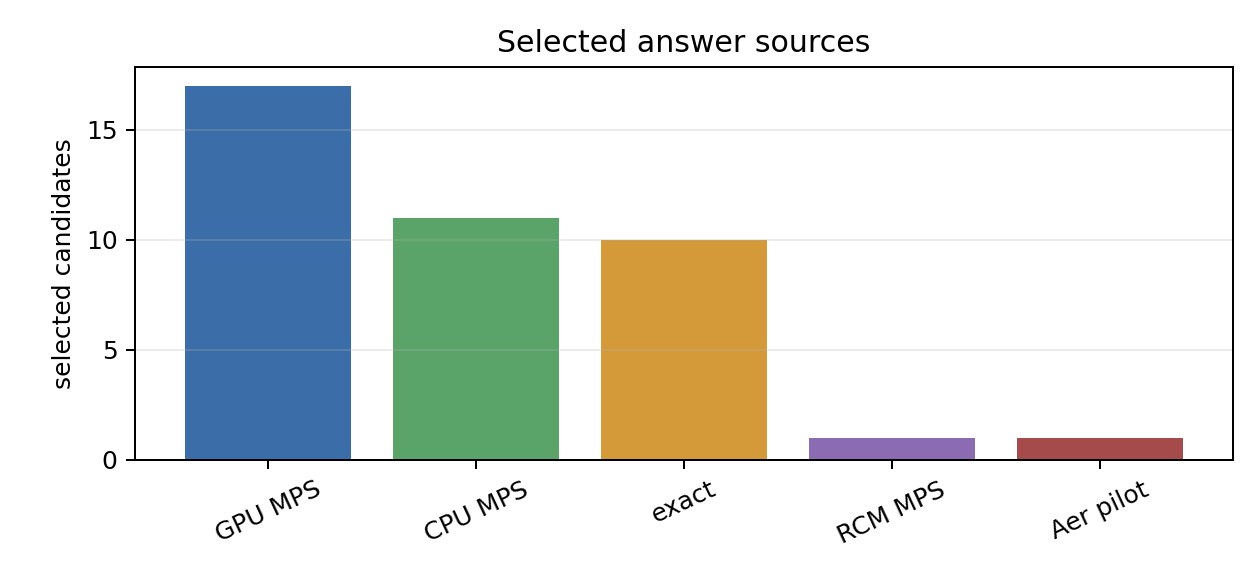
\includegraphics[width=0.68\linewidth]{figures/coverage_by_source.png}
  \caption{Selected candidate source counts in the current rollup.}
  \label{fig:sources}
\end{figure}

Figure~\ref{fig:runtime} summarizes peak strength and runtime for selected evidence. The easy and very-easy circuits usually have a visible sample peak, while several hard rows have very low observed top fractions. Those hard-row candidates should be treated as provisional until corroborated by the MPO-unswapping pass or another stronger method.

\begin{figure}[H]
  \centering
  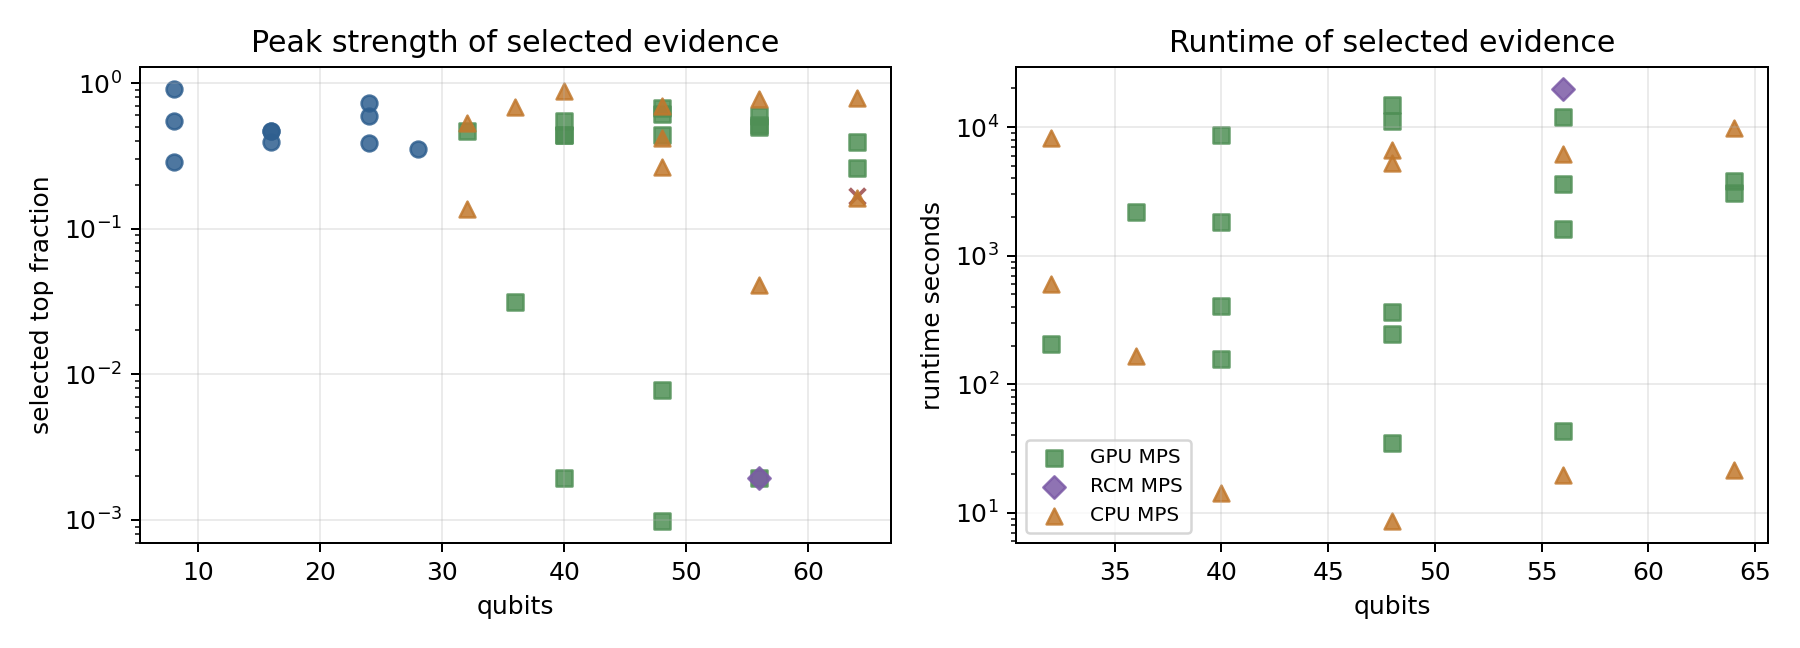
\includegraphics[width=0.95\linewidth]{figures/top_fraction_runtime.png}
  \caption{Selected evidence top fraction and runtime. Both axes use logarithmic scaling where appropriate. Exact rows have no runtime in this plot.}
  \label{fig:runtime}
\end{figure}

\section*{Representative Distributions}

Figure~\ref{fig:dist} compares representative sampled distributions. \texttt{40\_17} is a typical easy case: the peak dominates the sample. \texttt{56\_39} and \texttt{56\_38} show why the remaining hard tail was problematic for the MPS approach: the observed top count is only one or two samples out of hundreds or thousands, so the chosen bitstring is much less stable. The \texttt{16\_28} MPO-unswapping validation shows that the new path can recover the correct known answer quickly after applying the validated bit-order convention.

\begin{figure}[H]
  \centering
  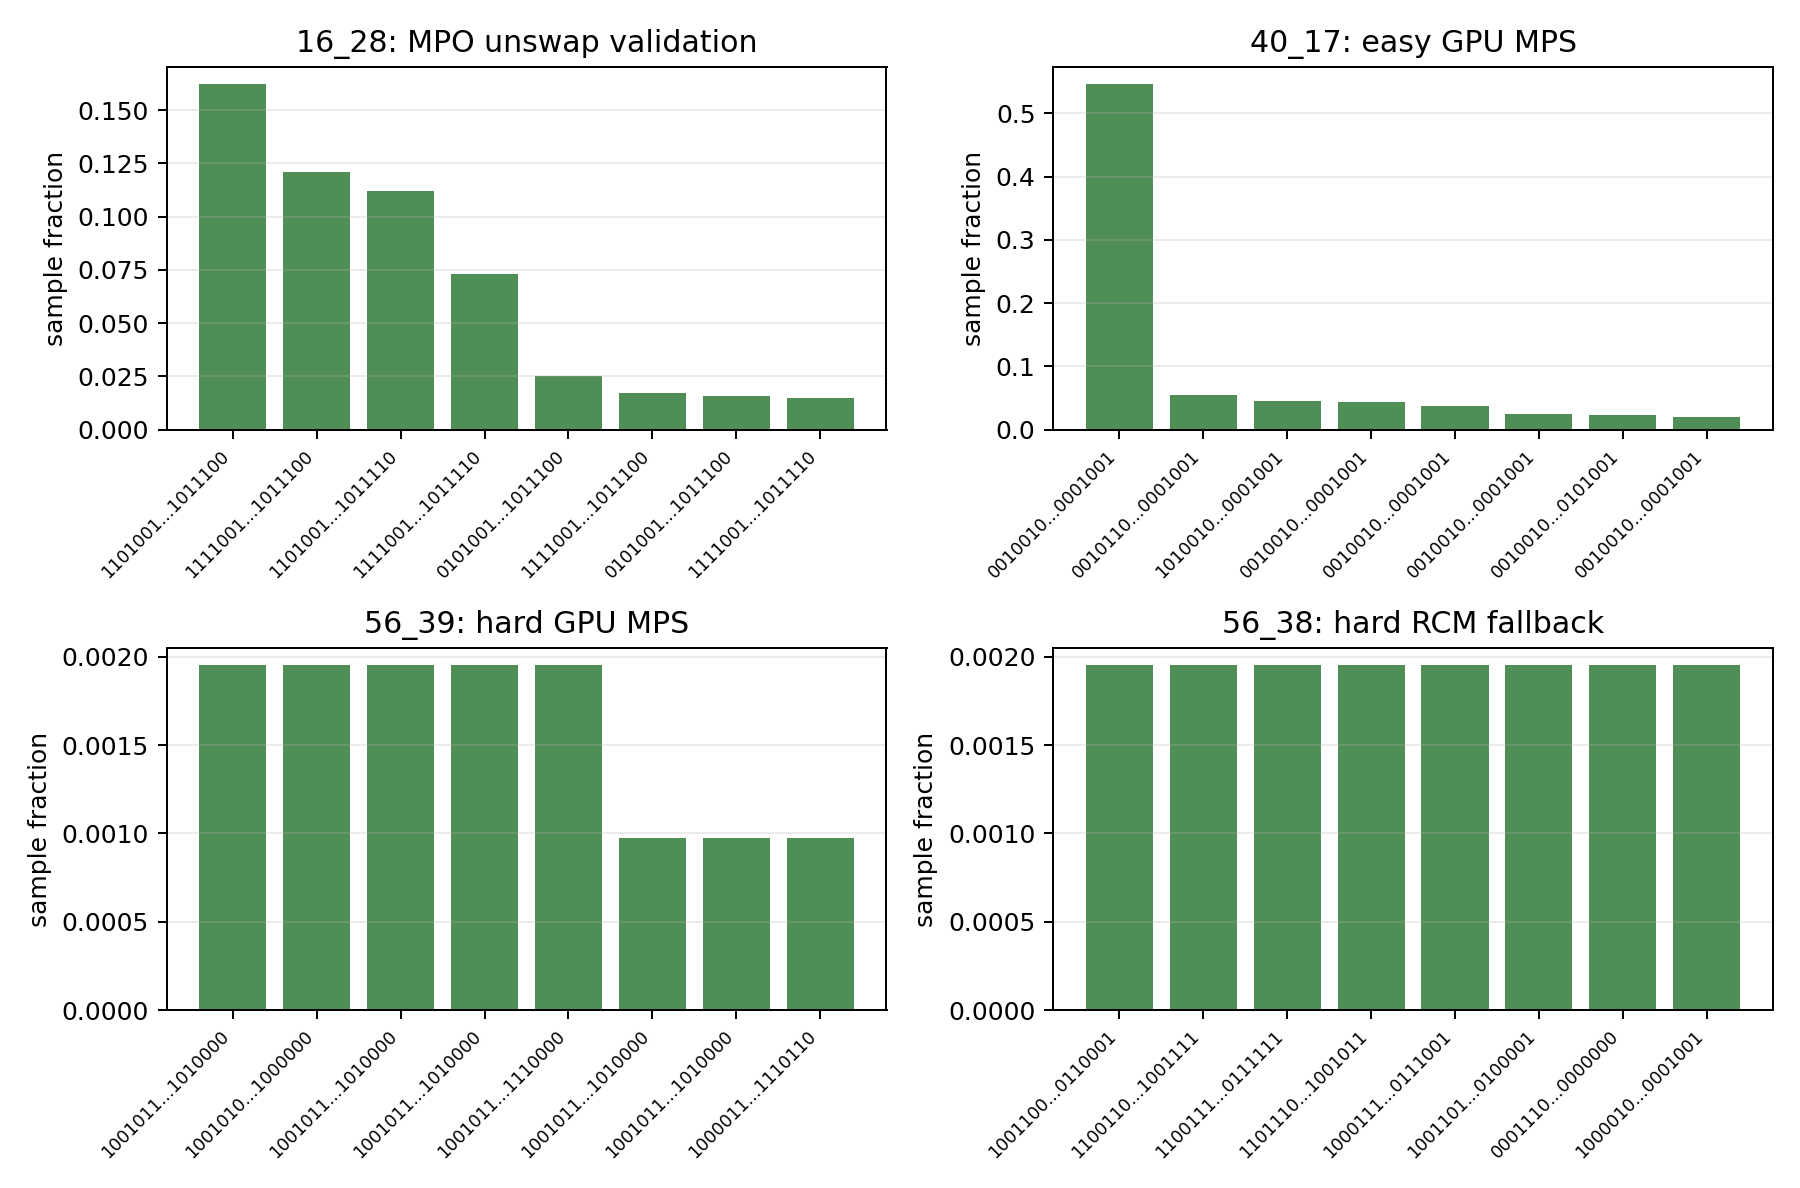
\includegraphics[width=0.95\linewidth]{figures/sample_distributions.png}
  \caption{Top sampled bitstring fractions for representative completed runs. Bitstring labels are shortened for readability.}
  \label{fig:dist}
\end{figure}

\section*{Notable Evidence}

\begin{itemize}
  \item \texttt{16\_28}: exact answer \texttt{1101001111011100}. The MPO-unswapping validation also produced this answer in 93.26 seconds, confirming the bit-order convention.
  \item \texttt{48\_37}: GPU and CPU graph-MPS agreed on the same 48-bit answer; the observed top fraction was only \texttt{0.0009765625}.
  \item \texttt{56\_38}: first filled by RCM CPU fallback; this is currently a weak fallback with top fraction \texttt{0.001953125}.
  \item \texttt{56\_39}: initially filled by degree-order fallback, then replaced by higher-priority GPU graph-MPS; top fraction remains only \texttt{0.001953125}.
  \item \texttt{64\_41}: filled only by the older Aer pilot with an unstable classification. It is included because it is currently the only candidate evidence for that label.
\end{itemize}

\section*{Current Caveats}

This is not yet a completed challenge solution. The report snapshot is 40/49. The unresolved MPO-unswapping array is active and may change the final rollup. The hard-tail MPS candidates with tiny top fractions are useful as placeholders and diagnostics, but they are not as trustworthy as exact rows or high-top-fraction MPS rows.

The main technical lesson from this session is that naive or graph-ordered MPS is not enough for the very-hard tail. The remaining circuits are dense RX/RZ/CX circuits with no explicit SWAPs, so the useful structure is likely hidden mirrored cancellation/permutation rather than a simple qubit-line ordering. The MPO iterative cancellation with unswapping is the right next path, and early validation shows it is compatible after the Quimb API and bit-order fixes.

\section*{Candidate Tables}

The following tables are generated directly from \texttt{outputs/tree\_tensor\_sim/collector\_current/CANDIDATES.tsv} at report-build time.

\newcommand{\ReportGenerated}{2026-06-06 06:31:01 BST}
\newcommand{\SelectedCount}{40}
\newcommand{\TotalCount}{49}
\newcommand{\UnresolvedList}{64\_40, 104\_49, 48\_42, 56\_43, 64\_44, 72\_45, 80\_46, 88\_47, 96\_48}

\begin{tabular}{lrr}
\toprule
Difficulty & selected & total \\
\midrule
easy & 16 & 16 \\
hard & 6 & 7 \\
moderate & 8 & 8 \\
very easy & 10 & 10 \\
very\_hard & 0 & 8 \\
\bottomrule
\end{tabular}

\bigskip

\begin{tabular}{lr}
\toprule
Source & selected \\ 
\midrule
GPU MPS & 17 \\
CPU MPS & 11 \\
exact & 10 \\
RCM MPS & 1 \\
Aer pilot & 1 \\
\bottomrule
\end{tabular}

\bigskip

\begin{longtable}{p{0.10\linewidth}p{0.12\linewidth}rp{0.39\linewidth}p{0.13\linewidth}r}
\caption{Current candidate rollup. Empty candidate rows are unresolved at report time.}\\
\toprule
Challenge & difficulty & q & candidate & source & top frac \\
\midrule
\endfirsthead
\toprule
Challenge & difficulty & q & candidate & source & top frac \\
\midrule
\endhead
\texttt{16\_12} & easy & 16 & {\scriptsize\ttfamily 11110001\allowbreak 01101011} & exact & 0.4665 \\
\texttt{24\_13} & easy & 24 & {\scriptsize\ttfamily 11111001\allowbreak 11110010\allowbreak 11010001} & exact & 0.5912 \\
\texttt{32\_14} & easy & 32 & {\scriptsize\ttfamily 00000101\allowbreak 00110100\allowbreak 00010111\allowbreak 11101100} & GPU MPS & 0.4717 \\
\texttt{36\_15} & easy & 36 & {\scriptsize\ttfamily 11011001\allowbreak 10111111\allowbreak 11011001\allowbreak 01111010\allowbreak 1111} & GPU MPS & 0.03125 \\
\texttt{40\_16} & easy & 40 & {\scriptsize\ttfamily 01011101\allowbreak 01001110\allowbreak 01100011\allowbreak 10111001\allowbreak 10010110} & GPU MPS & 0.4424 \\
\texttt{40\_17} & easy & 40 & {\scriptsize\ttfamily 00100101\allowbreak 01010111\allowbreak 00100100\allowbreak 00100010\allowbreak 00001001} & GPU MPS & 0.5459 \\
\texttt{40\_18} & easy & 40 & {\scriptsize\ttfamily 01000001\allowbreak 10010010\allowbreak 00110111\allowbreak 10001111\allowbreak 11001110} & GPU MPS & 0.4395 \\
\texttt{48\_19} & easy & 48 & {\scriptsize\ttfamily 01100101\allowbreak 01111011\allowbreak 00111110\allowbreak 00000101\allowbreak 11010011\allowbreak 10010000} & GPU MPS & 0.6738 \\
\texttt{48\_20} & easy & 48 & {\scriptsize\ttfamily 10101010\allowbreak 01010010\allowbreak 10000110\allowbreak 10100000\allowbreak 10111100\allowbreak 10000000} & GPU MPS & 0.6123 \\
\texttt{48\_21} & easy & 48 & {\scriptsize\ttfamily 11101010\allowbreak 11101010\allowbreak 11110101\allowbreak 00000110\allowbreak 10001000\allowbreak 00001001} & GPU MPS & 0.4414 \\
\texttt{56\_22} & easy & 56 & {\scriptsize\ttfamily 11100100\allowbreak 10011001\allowbreak 00111100\allowbreak 10110110\allowbreak 01100000\allowbreak 01000101\allowbreak 11111011} & GPU MPS & 0.5898 \\
\texttt{56\_23} & easy & 56 & {\scriptsize\ttfamily 01001101\allowbreak 00111111\allowbreak 11000001\allowbreak 01001110\allowbreak 11101110\allowbreak 00111111\allowbreak 00001101} & GPU MPS & 0.4971 \\
\texttt{56\_24} & easy & 56 & {\scriptsize\ttfamily 10011001\allowbreak 00111110\allowbreak 11111110\allowbreak 11101011\allowbreak 10110101\allowbreak 00110010\allowbreak 11110001} & GPU MPS & 0.5176 \\
\texttt{64\_25} & easy & 64 & {\scriptsize\ttfamily 00111011\allowbreak 11110000\allowbreak 11011011\allowbreak 11010110\allowbreak 00010000\allowbreak 01010011\allowbreak 01110000\allowbreak 01111011} & GPU MPS & 0.3965 \\
\texttt{64\_26} & easy & 64 & {\scriptsize\ttfamily 01101010\allowbreak 10100011\allowbreak 01011101\allowbreak 10000111\allowbreak 00010110\allowbreak 11011001\allowbreak 11000110\allowbreak 01100110} & GPU MPS & 0.2617 \\
\texttt{8\_11} & easy & 8 & {\scriptsize\ttfamily 01001110} & exact & 0.5454 \\
\texttt{40\_35} & hard & 40 & {\scriptsize\ttfamily 01011001\allowbreak 10101111\allowbreak 11100001\allowbreak 01010011\allowbreak 10001001} & GPU MPS & 0.001953 \\
\texttt{48\_36} & hard & 48 & {\scriptsize\ttfamily 00111101\allowbreak 10110011\allowbreak 00110011\allowbreak 00100010\allowbreak 10011010\allowbreak 10111000} & GPU MPS & 0.007812 \\
\texttt{48\_37} & hard & 48 & {\scriptsize\ttfamily 10010100\allowbreak 10100011\allowbreak 01010100\allowbreak 10010100\allowbreak 10010001\allowbreak 01010001} & GPU MPS & 0.0009766 \\
\texttt{56\_38} & hard & 56 & {\scriptsize\ttfamily 10011001\allowbreak 01111000\allowbreak 00000100\allowbreak 11010101\allowbreak 10000100\allowbreak 10011101\allowbreak 10110001} & RCM MPS & 0.001953 \\
\texttt{56\_39} & hard & 56 & {\scriptsize\ttfamily 10010111\allowbreak 00110101\allowbreak 01011111\allowbreak 11010110\allowbreak 11011011\allowbreak 00001010\allowbreak 01010000} & GPU MPS & 0.001953 \\
\texttt{64\_40} & hard & 64 & -- & blank &  \\
\texttt{64\_41} & hard & 64 & {\scriptsize\ttfamily 00010001\allowbreak 11010011\allowbreak 10011001\allowbreak 00111101\allowbreak 11000000\allowbreak 10001101\allowbreak 00011010\allowbreak 10110010} & Aer pilot & 0.167 \\
\texttt{16\_28} & moderate & 16 & {\scriptsize\ttfamily 11010011\allowbreak 11011100} & exact & 0.3962 \\
\texttt{24\_29} & moderate & 24 & {\scriptsize\ttfamily 11010001\allowbreak 01111000\allowbreak 01001001} & exact & 0.3901 \\
\texttt{32\_30} & moderate & 32 & {\scriptsize\ttfamily 10011000\allowbreak 01001111\allowbreak 01111011\allowbreak 11010111} & CPU MPS & 0.1357 \\
\texttt{48\_31} & moderate & 48 & {\scriptsize\ttfamily 10110011\allowbreak 10001010\allowbreak 11111111\allowbreak 10101011\allowbreak 10110110\allowbreak 00110110} & CPU MPS & 0.4209 \\
\texttt{48\_32} & moderate & 48 & {\scriptsize\ttfamily 01110101\allowbreak 01110111\allowbreak 10001110\allowbreak 01010101\allowbreak 01011011\allowbreak 10001110} & CPU MPS & 0.2656 \\
\texttt{56\_33} & moderate & 56 & {\scriptsize\ttfamily 11001001\allowbreak 10010100\allowbreak 11110101\allowbreak 00100010\allowbreak 01010111\allowbreak 11110111\allowbreak 01010000} & CPU MPS & 0.04102 \\
\texttt{64\_34} & moderate & 64 & {\scriptsize\ttfamily 00110101\allowbreak 00010011\allowbreak 00111010\allowbreak 11101001\allowbreak 01001011\allowbreak 00101101\allowbreak 10011110\allowbreak 11100110} & CPU MPS & 0.1631 \\
\texttt{8\_27} & moderate & 8 & {\scriptsize\ttfamily 11001001} & exact & 0.2879 \\
\texttt{16\_2} & very easy & 16 & {\scriptsize\ttfamily 10101010\allowbreak 11001000} & exact & 0.467 \\
\texttt{24\_3} & very easy & 24 & {\scriptsize\ttfamily 01111001\allowbreak 00001010\allowbreak 10001000} & exact & 0.724 \\
\texttt{28\_4} & very easy & 28 & {\scriptsize\ttfamily 11111110\allowbreak 00101010\allowbreak 11011001\allowbreak 1111} & exact & 0.3511 \\
\texttt{32\_5} & very easy & 32 & {\scriptsize\ttfamily 00111000\allowbreak 10101010\allowbreak 00010000\allowbreak 00010000} & CPU MPS & 0.5322 \\
\texttt{36\_6} & very easy & 36 & {\scriptsize\ttfamily 10011010\allowbreak 01111010\allowbreak 01001101\allowbreak 11001100\allowbreak 1000} & CPU MPS & 0.6885 \\
\texttt{40\_7} & very easy & 40 & {\scriptsize\ttfamily 01101110\allowbreak 11010001\allowbreak 01001111\allowbreak 11100100\allowbreak 11000111} & CPU MPS & 0.8789 \\
\texttt{48\_8} & very easy & 48 & {\scriptsize\ttfamily 00010010\allowbreak 01101110\allowbreak 01001111\allowbreak 11110010\allowbreak 10110011\allowbreak 10010100} & CPU MPS & 0.6973 \\
\texttt{56\_9} & very easy & 56 & {\scriptsize\ttfamily 10010110\allowbreak 10110010\allowbreak 11101001\allowbreak 10010110\allowbreak 01110110\allowbreak 01100011\allowbreak 01010100} & CPU MPS & 0.7812 \\
\texttt{64\_10} & very easy & 64 & {\scriptsize\ttfamily 00110100\allowbreak 10110001\allowbreak 11001011\allowbreak 10011001\allowbreak 00101100\allowbreak 01011111\allowbreak 01100101\allowbreak 00101011} & CPU MPS & 0.7871 \\
\texttt{8\_1} & very easy & 8 & {\scriptsize\ttfamily 10101101} & exact & 0.9126 \\
\texttt{104\_49} & very\_hard & 104 & -- & blank &  \\
\texttt{48\_42} & very\_hard & 48 & -- & blank &  \\
\texttt{56\_43} & very\_hard & 56 & -- & blank &  \\
\texttt{64\_44} & very\_hard & 64 & -- & blank &  \\
\texttt{72\_45} & very\_hard & 72 & -- & blank &  \\
\texttt{80\_46} & very\_hard & 80 & -- & blank &  \\
\texttt{88\_47} & very\_hard & 88 & -- & blank &  \\
\texttt{96\_48} & very\_hard & 96 & -- & blank &  \\
\bottomrule
\end{longtable}


\end{document}
